\documentclass[12pt]{article} 

\usepackage{amsmath, amssymb, amsfonts}
\usepackage[bottom=2.0cm, right=2.0cm, left=2.0cm, top=2.0cm]{geometry}
\usepackage{graphicx}
\usepackage{tikz}
\usepackage{hyperref}
\usepackage{xcolor}
\usepackage{listings}
\usepackage{titlesec}
\usepackage{hyperref}
\graphicspath{{./images/}}
%\pagenumbering{gobble}
\parindent 0px

\title{GUIDE: Running Models on Gcloud}
\author{CMPT419: PROJECT19}
\date{}
%SetFonts

\setcounter{tocdepth}{4}
\setcounter{secnumdepth}{4}

\titleformat{\paragraph}
{\normalfont\normalsize\bfseries}{\theparagraph}{1em}{}
\titlespacing*{\paragraph}
{0pt}{3.25ex plus 1ex minus .2ex}{1.5ex plus .2ex}

%SetFonts

% Define a style for command-line input
\lstdefinestyle{custombash}{
    language=bash,
    backgroundcolor=\color{gray!10},
    basicstyle=\ttfamily\small,
    breaklines=true,
    showstringspaces=false,
    commentstyle=\color{gray},
    columns=fullflexible
}
\lstdefinestyle{custombash2}{
    language=bash,
    backgroundcolor=\color{gray!10},
    basicstyle=\ttfamily\tiny,
    breaklines=true,
    showstringspaces=false,
    commentstyle=\color{gray},
    columns=fullflexible
}

\begin{document}
\maketitle
\vspace{-1cm}

\section{Renting a GPU}
While there are multiple websites available where you can rent NVIDIA GPUs. It is suggested you use Google Cloud Console since it offers $\approx\$400$ worth of free credits (this is more than enough for our usage). Also note that before beggining, you should install Google CLI on your local computer. Refer to \href{https://cloud.google.com/sdk/docs/install}{installation instructions}.\\

\subsection{Creating Account and increasing Quota}
\begin{itemize}
	\item
	Go to \href{https://cloud.google.com}{GCP's homepage} and select- `Get Started for Free'.
	
	\item
	Follow the signup instructions and you should receive free credits automatically.
	
	\item
	Go to \href{https://console.cloud.google.com/}{Google Cloud Console} and start a project (you might also have to setup billing information to keep your free credits from getting expired).
	
	\item
	Head to \href{https://console.cloud.google.com/iam-admin/quotas?_ga=2.43326246.2094772927.1720406019-760686455.1700081600&_gac=1.222441065.1720474391.CjwKCAjwnK60BhA9EiwAmpHZw9FxhNBMBVr07uVS5tzDRUb2l4nRARWjSuvP0NW8KQjphSTtuKyUAxoC0W8QAvD_BwE}{Quotas} page on GCP and select `Compute Engine API'
	
	\item
	Under the `Compute Engine API (Networks)', increase the limit for `gpus(all region)' and `L4' (since we are using `L4' in our case) gpus for your preferred locations. For example, the increase requests may look as given in Figure1  
    \ref{fig:gpu_request}

	\begin{figure}
    	\centering
   		 \begin{tikzpicture}
        		\node[inner sep=0pt] (image) at (0,0) {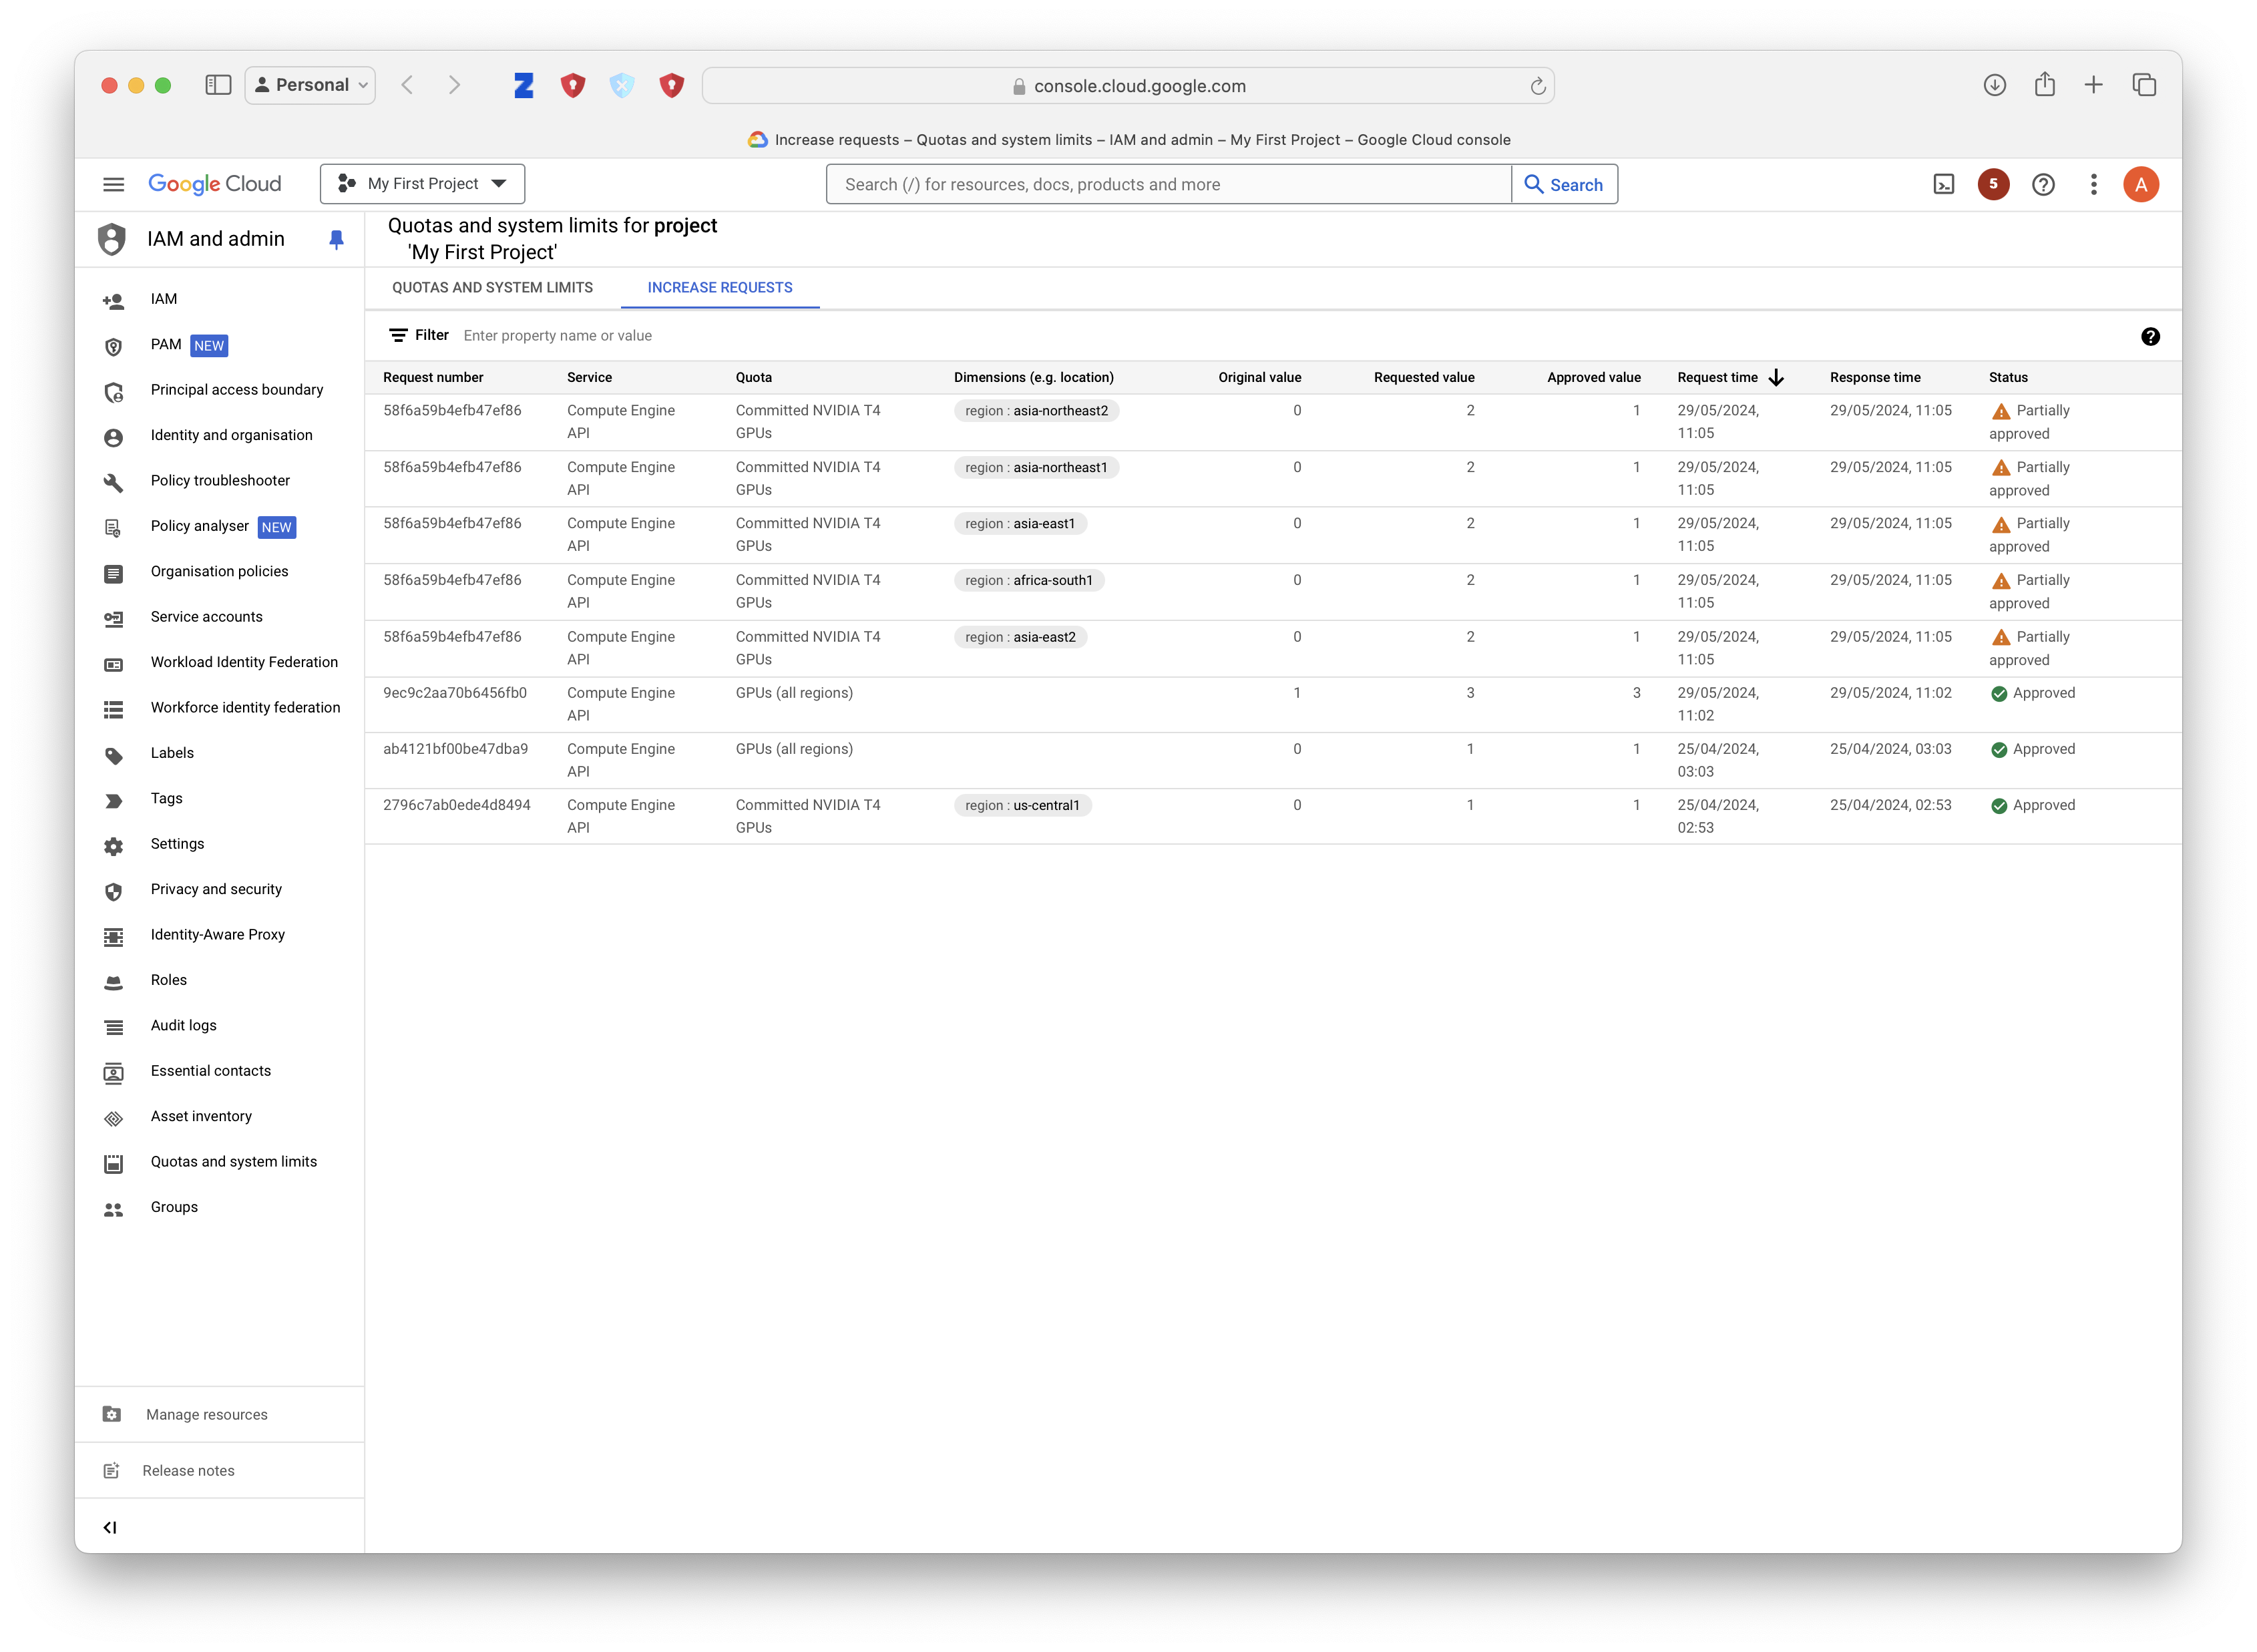
\includegraphics[scale=0.22]{gpu_request}};
        		\draw[red, thick] (image.south west) rectangle (image.north east);
    		\end{tikzpicture}
    		\caption{Increase Requests on GCP}
            \label{fig:gpu_request}
	\end{figure}
	
\end{itemize}

\subsection{Creating a VM}

\begin{itemize}
	\item
	Head to \href{https://console.cloud.google.com/}{\color{blue}Google Cloud Console} and select `Compute Engine' after logging in. 
	
	\item
	Click `Create Instance' from the top menu.
	
	\item
	Name the instance and select a region.
	
	\item
	Under the `Machine Configuration', select `GPUs' and choose one ` NVIDIA L4' GPU.
		
	\item
	Leaving other settings as they are, under the `Boot Disk' menu, select `Change' and modify the OS to `Ubuntu' with version `x86/64 22.04 LTS`. Lastly, change the size of the disk to 100 GB for now. You may increase the it later.
	
	\item
	After all of the above steps, select `Create'. If the GPU is available in the region, the google cloud platform will create it in a few minutes, ready to use.
\end{itemize}

\textbf{Note}, if you see an error mentioning `GPUs unavailable in selected region', redo the whole process with different region selected. 


\subsection{Connecting to VM}
There are multiple ways to connect to the created VM. It is recommended you use your own local terminal and ssh into it since connection through other methods expire after inactivity. \\

For \textbf{SSH} connection,

\begin{itemize}
	\item
	Click the dropdown arrow under `Connect' and from the available options, select `View gcloud command'
	\begin{figure}[h]
    	\centering
   		 \begin{tikzpicture}
        		\node[inner sep=0pt] (image) at (0,0) {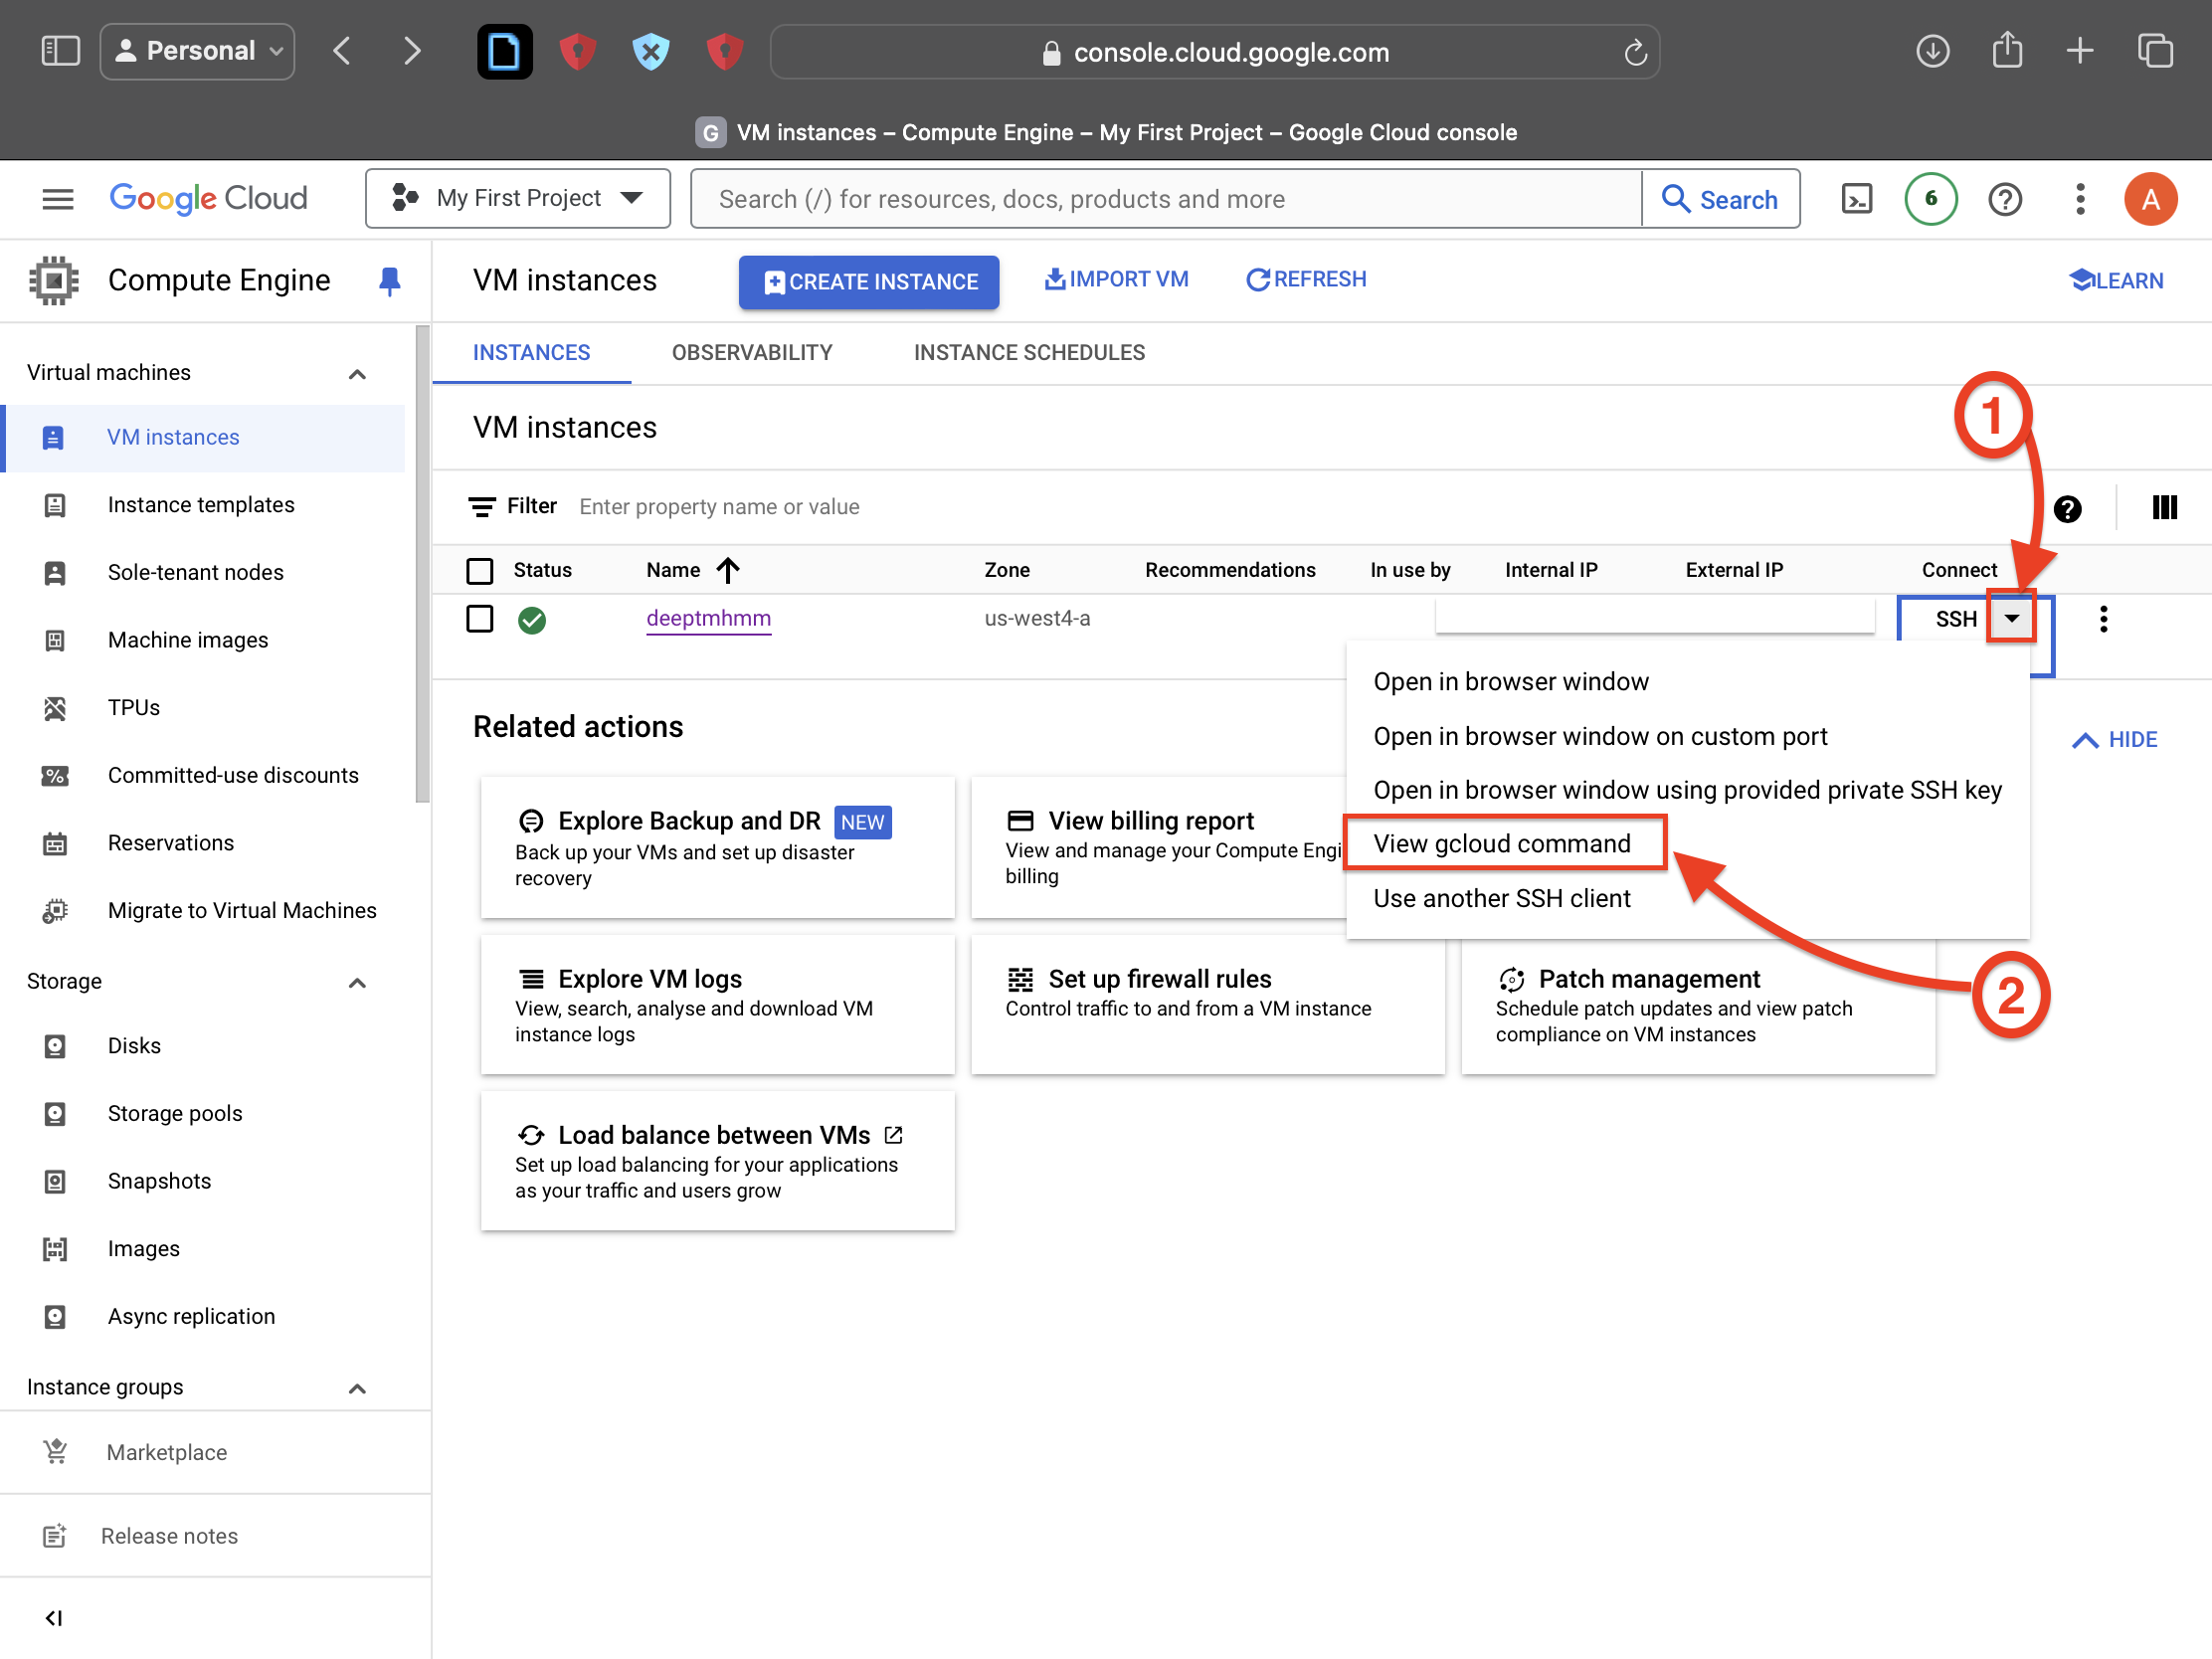
\includegraphics[scale=0.20]{ssh_cmd}};
        		\draw[red, thick] (image.south west) rectangle (image.north east);
    		\end{tikzpicture}
    		\caption{Selecting gcloud Command}
	\end{figure}
	
	\item
	Copy the displayed command and enter it in your \textbf{LOCAL} terminal.
\end{itemize}

You should now have successfully established a connection with the VM through your terminal.

\subsection{Using VM w/ Remote SSH on Vscode}
If you are using VScode, you can also connect to the VM using the Remote SSH extension. This allows you to use the GUI of VScode to run commands on the VM.\\

To do so, follow the steps below-
\begin{itemize}
    \item
    Install the Remote SSH extension on VScode.
    
    \item
    Open the command palette (Ctrl + Shift + P) and select `Remote-SSH: Connect to Host...'
    
    \item
    Paste the gcloud command you copied earlier in the input box and hit enter.
    
    \item
    VScode will now connect to the VM and open a new window with the remote file system.

    \item
    You can now use the terminal in VScode to run commands on the VM.
\end{itemize}

See the figure below for verifying the connection-
\begin{figure}[h]
    \centering
        \begin{tikzpicture}
            \node[inner sep=0pt] (image) at (0,0) {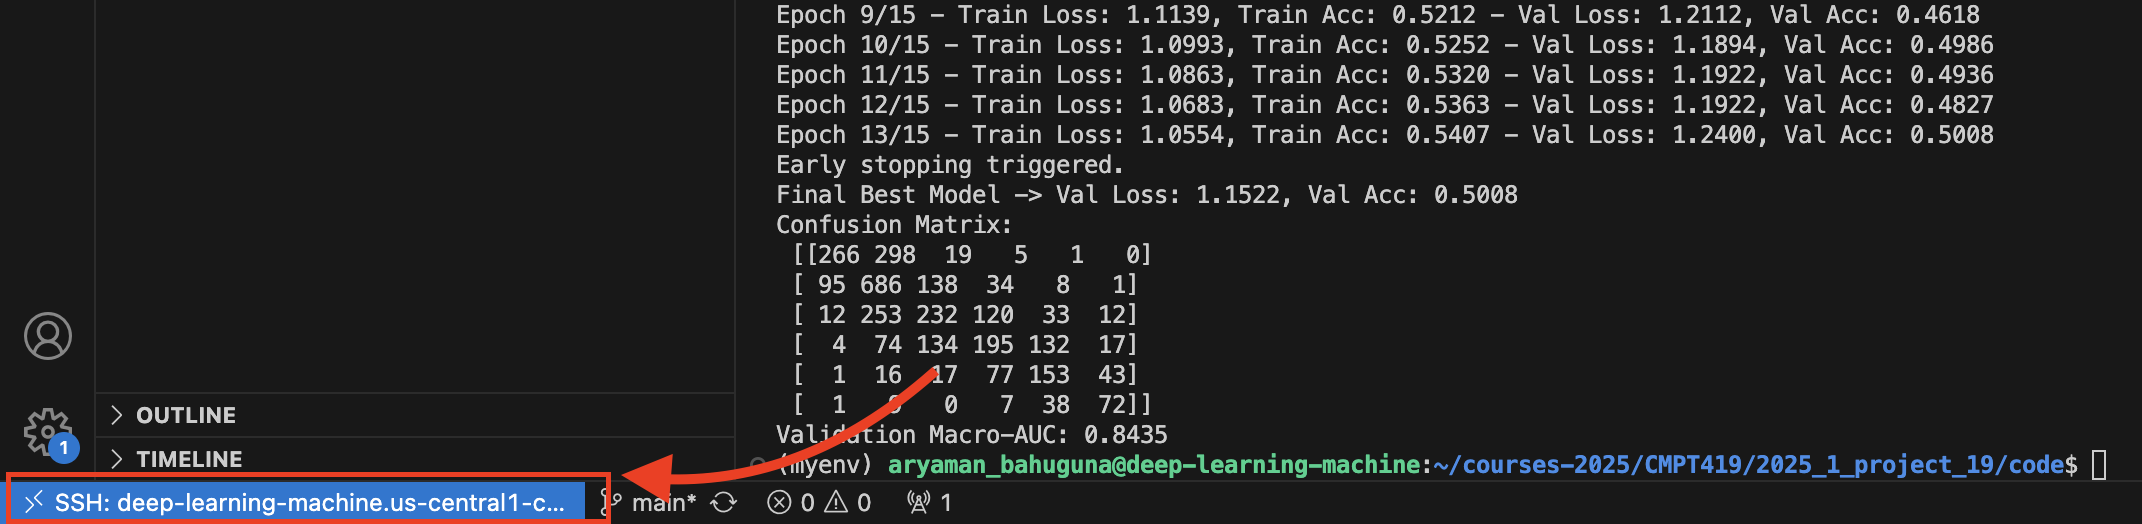
\includegraphics[scale=0.40]{vscode-connection}};
            \draw[red, thick] (image.south west) rectangle (image.north east);
        \end{tikzpicture}
        \caption{VScode Connection}
\end{figure}

\section{Installing GPU Drivers}
\label{sec:hello}
After setting up the VM, GPU drivers must be installed. Refer Compute Engine Documentation- \href{https://cloud.google.com/compute/docs/gpus/install-drivers-gpu}{\color{blue}Install GPU Drivers}. (Before beggining, ensure you are ssh'd into the VM)

\section{TEST: Running Models on Gcloud VM}
You may now clone the repository from \href{Github}{Github-Repo-Link} and run our results on the VM. The datasets link is: \href{no-link}{\color{blue}Google Drive Link}.\\

\end{document}  